\chapter{Data and Methodology}
\label{chap:met}

\section{Raw Data}

	The data originates from two sources. The first and most important source is Thomson Reuters Datastream. It covers publicly traded shares from developed countries of Europe, Japan and Asia-Pacific (Australia, New Zealand, Hong Kong, and Singapore) and contains the firms' yearly accounting figures and daily market information (e.g., price and volume).  The second data source is Institutional Brokers’ Estimate System (I/B/E/S) from Wharton Research Data Services, which provides analysts' forecasts. 
	
	The firms are filtered based on [TODO add source of filtering methods].  
	The final sample includes 8350 companies.


\section{Anomalies Data}
	The anomaly dataset consists of 153 anomalies published in leading financial and accounting journals. The data is monthly and spans from January 1990 to December 2018. It covers the same 8350 firms as the raw data, totaling 1,607,117 observations. 
	
	The anomalies can be classified into three groups: Fundamentals, Frictions, and I/B/E/S anomalies. Fundamental anomalies are primarily calculated from yearly accounting statements and are exemplified by Total Accruals, Asset Growth, or Leverage. Fundamental anomalies fall into 5 broad categories: Accruals (e.g., Total Accruals, Change in Common Equity, Inventory Growth), Investment (e.g., Asset Growth, Debt Issuance, Net Operating Assets), Intangibles (e.g., Asset Liquidity, Earnings Persistence, Herfindahl Index), Profitability (e.g., Profit Margin, Return-on-Equity, Capital Turnover) and Value (e.g., Enterprise Multiple, Assets-to-Market, or Net Payout Yield). Friction anomalies are primarily calculated from daily market data. For example, they include Bid-Ask Spread, 11-Month Residual Momentum, 52-Week-High, and Long-Term Reversal. I/B/E/S anomalies are calculated from the I/B/E/S dataset and cover analysts' forecasts and recommendations, such as Analyst Value, Change in Recommendation, or Forecast Dispersion. There are 93 Fundamentals, 48 Frictions and 12 I/B/E/S anomalies. Within the Fundamentals category, there are 21 Accruals, 15 Investment, 25 Intangibles, 18 Profitability, and 14 Value anomalies.  
	
	A complete list of the anomalies can be found in the Appendix. [TODO]. 
	
	Tables \ref{tab:descr_fund}, \ref{tab:descr_frictions}, and \ref{tab:descr_ibes} show descriptive statistics of the anomalies data. [TODO fit too long fund table to page or split across multiple pages.]
		
	Figures \ref{fig:corrplot_funds}, \ref{fig:corrplot_frictions}, and \ref{fig:corrplot_ibes} show plots of correlation matrices of Fundamental, Frictions, and I/B/E/S anomalies respectively. Correlations between variables from different categories are not shown, as they are all very low but for negligible exceptions. 

	Figure \ref{fig:hist_returns} shows histogram of monthly returns. 
	

	%\begin{tabular}{lrrrrrrrr}
\toprule
{} &      count &  mean &     std &     min &     25\% &     50\% &     75\% &    max \\
\midrule
Lagged Momentum                            &  1607088.0 &   0.0 &  0.0316 & -0.1518 & -0.0053 & -0.0009 &  0.0029 &  1.000 \\
Seasonality                                &  1607088.0 &  -0.0 &  0.0282 & -0.2622 & -0.0034 & -0.0002 &  0.0021 &  1.000 \\
Short-Term Reversal                        &  1607088.0 &  -0.0 &  0.2430 & -0.9831 & -0.1276 & -0.0178 &  0.1027 &  1.000 \\
Momentum-Reversal                          &  1607088.0 &   0.0 &  0.0200 & -0.0802 & -0.0054 & -0.0008 &  0.0029 &  1.000 \\
52-Week High                               &  1607088.0 &  -0.0 &  0.3316 & -1.0000 & -0.1828 &  0.0764 &  0.2445 &  0.678 \\
RD / Market Equity                         &  1607088.0 &  -0.0 &  0.0169 & -0.0311 & -0.0001 &  0.0000 &  0.0000 &  1.000 \\
Liquidity Shocks                           &  1607088.0 &  -0.0 &  0.0055 & -0.0016 & -0.0001 & -0.0001 & -0.0000 &  1.000 \\
Earnings Predictability                    &  1607088.0 &   0.0 &  0.0158 & -0.0081 & -0.0006 &  0.0000 &  0.0000 &  1.000 \\
Seasonality 6-10 A                         &  1607088.0 &  -0.0 &  0.0220 & -0.1208 & -0.0055 &  0.0000 &  0.0029 &  1.000 \\
Change in Common Equity                    &  1607088.0 &  -0.0 &  0.0153 & -0.0199 & -0.0013 & -0.0003 & -0.0001 &  1.000 \\
Seasonality 6-10 N                         &  1607088.0 &   0.0 &  0.0220 & -0.1307 & -0.0050 &  0.0000 &  0.0020 &  1.000 \\
Seasonality 2-5 N                          &  1607088.0 &   0.0 &  0.0219 & -0.1313 & -0.0061 & -0.0005 &  0.0035 &  1.000 \\
Seasonality 2-5 A                          &  1607088.0 &  -0.0 &  0.0180 & -0.1002 & -0.0042 & -0.0000 &  0.0027 &  1.000 \\
Leverage Component of Book/Price           &  1607088.0 &   0.0 &  0.0089 & -0.0057 & -0.0002 & -0.0001 & -0.0000 &  1.000 \\
Amihud's Measure (Illiquidity)             &  1607088.0 &   0.0 &  0.0221 & -0.0113 & -0.0005 & -0.0002 & -0.0001 &  1.000 \\
Profit Margin                              &  1607088.0 &   0.0 &  0.0652 & -1.0000 & -0.0000 &  0.0011 &  0.0097 &  1.000 \\
Volume Trend                               &  1607088.0 &   0.0 &  0.2040 & -0.8532 & -0.0873 &  0.0000 &  0.0979 &  1.000 \\
Coefficient of Variation of Share Turnover &  1607088.0 &  -0.0 &  0.1144 & -0.1469 & -0.0625 & -0.0279 &  0.0170 &  1.000 \\
Earnings Forecast-to-Price                 &  1607088.0 &   0.0 &  0.0137 & -0.1066 & -0.0006 &  0.0000 &  0.0000 &  1.000 \\
Duration of Equity                         &  1607088.0 &   0.0 &  0.0624 & -1.0000 & -0.0006 &  0.0000 &  0.0068 &  1.000 \\
Seasonality 11-15 N                        &  1607088.0 &   0.0 &  0.0213 & -0.1246 & -0.0032 &  0.0000 &  0.0005 &  1.000 \\
Operating Profits to Assets                &  1607088.0 &   0.0 &  0.0562 & -0.3581 & -0.0122 &  0.0000 &  0.0011 &  1.000 \\
Max                                        &  1607088.0 &   0.0 &  0.1913 & -0.2571 & -0.1111 & -0.0544 &  0.0416 &  1.000 \\
Whited-Wu Index                            &  1607088.0 &   0.0 &  0.1681 & -0.7012 & -0.0528 &  0.0000 &  0.0489 &  1.000 \\
Net Operating Assets                       &  1607088.0 &  -0.0 &  0.0171 & -0.0869 & -0.0007 & -0.0001 &  0.0000 &  1.000 \\
Accruals                                   &  1607088.0 &   0.0 &  0.0484 & -0.3996 & -0.0043 &  0.0000 &  0.0033 &  1.000 \\
Idiosyncratic Risk                         &  1607088.0 &  -0.0 &  0.1999 & -0.2929 & -0.1204 & -0.0539 &  0.0528 &  1.000 \\
Coskewness                                 &  1607088.0 &  -0.0 &  0.1996 & -1.0000 & -0.1014 &  0.0000 &  0.1074 &  1.000 \\
Liquidity Beta 5                           &  1607088.0 &  -0.0 &  0.0724 & -0.3288 & -0.0298 &  0.0000 &  0.0213 &  1.000 \\
Liquidity Beta 3                           &  1607088.0 &  -0.0 &  0.0568 & -0.3347 & -0.0100 &  0.0000 &  0.0204 &  1.000 \\
\bottomrule
\end{tabular}

	
	\begin{table}
		\resizebox{\textwidth}{!}{\begin{tabular}{lrrrrrrrr}
\toprule
{} &      count &          mean &           std &           min &        25\% &        50\% &        75\% &           max \\
\midrule
Accr      &  1326726.0 & -3.130000e-02 &  3.010000e-01 & -5.376980e+01 &    -0.0668 &    -0.0299 &     0.0045 &  2.323860e+01 \\
AGr       &  1426822.0 &           inf &           NaN & -1.000000e+00 &    -0.0557 &     0.0595 &     0.1852 &           inf \\
AL        &  1185337.0 &          -inf &           NaN &          -inf &    -0.6710 &    -0.5098 &    -0.3670 &  1.196750e+01 \\
AL2       &  1135791.0 & -1.078751e+03 &  1.791780e+05 & -4.988183e+07 &    -1.5728 &    -0.7994 &    -0.3784 &  4.935200e+00 \\
ATurn     &  1174246.0 &  3.595700e+00 &  1.478946e+02 & -4.632576e+03 &     0.8766 &     1.6008 &     2.7225 &  2.580516e+04 \\
AtM       &  1463723.0 &  4.043164e+03 &  8.896111e+05 &  0.000000e+00 &     0.8506 &     1.6844 &     3.5502 &  2.202320e+08 \\
BM        &  1443483.0 &          -inf &           NaN &          -inf &    -1.0495 &    -0.4264 &     0.1646 &  1.494580e+01 \\
CT        &  1424872.0 &           inf &           NaN & -9.138000e-01 &     0.3921 &     0.8189 &     1.2702 &           inf \\
CFoMV     &  1358488.0 &  3.053290e+01 &  3.733290e+03 & -3.856522e+04 &     0.0401 &     0.0865 &     0.1531 &  8.549874e+05 \\
CBOP      &  1044783.0 &          -inf &           NaN &          -inf &     0.0348 &     0.0902 &     0.1541 &  5.517662e+03 \\
CtA       &  1356655.0 &  1.735000e-01 &  1.610000e-01 &  0.000000e+00 &     0.0611 &     0.1275 &     0.2321 &  2.461500e+00 \\
dATurn    &  1011919.0 & -2.033000e-01 &  2.720040e+01 & -2.582384e+03 &    -0.2043 &    -0.0190 &     0.1081 &  3.323493e+03 \\
dCE       &  1426774.0 &           inf &           NaN & -8.540260e+03 &    -0.0156 &     0.0209 &     0.0796 &           inf \\
dCOA      &  1219678.0 &           inf &           NaN & -3.769400e+00 &    -0.0216 &     0.0128 &     0.0631 &           inf \\
dCOL      &  1220041.0 &          -inf &           NaN &          -inf &    -0.0191 &     0.0091 &     0.0475 &  2.031640e+07 \\
dFL       &  1425235.0 &          -inf &           NaN &          -inf &    -0.0248 &     0.0000 &     0.0472 &  2.488448e+07 \\
dLTI      &   852533.0 &  1.010000e-01 &  2.134350e+01 & -9.762000e-01 &    -0.0033 &     0.0000 &     0.0071 &  6.969071e+03 \\
dNFA      &  1136823.0 &           inf &           NaN & -2.488448e+07 &    -0.0587 &    -0.0006 &     0.0436 &           inf \\
dNNCWC    &  1219392.0 &           inf &           NaN & -1.933512e+07 &    -0.0247 &     0.0031 &     0.0350 &           inf \\
dNNCOA    &  1219475.0 &           inf &           NaN & -1.142870e+03 &    -0.0260 &     0.0161 &     0.0750 &           inf \\
dNCOA     &  1219945.0 &           inf &           NaN & -1.496010e+01 &    -0.0258 &     0.0179 &     0.0795 &           inf \\
dNCOL     &  1219851.0 &           inf &           NaN & -2.223446e+05 &    -0.0048 &     0.0005 &     0.0090 &           inf \\
dPM       &  1265175.0 &           NaN &           NaN &          -inf &    -0.0133 &     0.0015 &     0.0178 &           inf \\
dSTI      &   970776.0 &  2.060000e-02 &  2.416700e+00 & -9.642000e-01 &    -0.0066 &     0.0000 &     0.0084 &  6.835770e+02 \\
ChNOA     &  1284565.0 &           inf &           NaN & -3.521843e+03 &    -0.0400 &     0.0312 &     0.1140 &           inf \\
ChPPEIA   &  1227511.0 &           inf &           NaN & -1.437410e+01 &    -0.0261 &     0.0329 &     0.1204 &           inf \\
CDI       &   667698.0 &           inf &           NaN & -9.899100e+00 &    -1.0154 &     0.0821 &     1.3740 &           inf \\
CEI5Y     &  1288644.0 &  1.125000e-01 &  6.540000e-01 & -1.139050e+01 &    -0.1206 &    -0.0373 &     0.1241 &  1.987440e+01 \\
DI        &  1468025.0 &  5.174000e-01 &  4.997000e-01 &  0.000000e+00 &     0.0000 &     1.0000 &     1.0000 &  1.000000e+00 \\
DA        &  1223877.0 & -5.800000e-03 &  7.217000e-01 & -1.100946e+02 &    -0.0409 &    -0.0004 &     0.0386 &  6.328230e+01 \\
DurE      &  1400768.0 &           NaN &           NaN &          -inf &    -4.9750 &     5.5412 &    11.6959 &           inf \\
ES        &   560569.0 &  2.560000e-02 &  1.424900e+00 &  0.000000e+00 &     0.0002 &     0.0005 &     0.0017 &  1.145981e+02 \\
EoP       &  1251646.0 &  3.200700e+01 &  3.668273e+03 &  0.000000e+00 &     0.0295 &     0.0524 &     0.0878 &  6.797906e+05 \\
ECon      &   802280.0 &  9.806000e-01 &  8.442385e+02 & -3.277065e+05 &     0.7819 &     1.1617 &     2.0798 &  5.903915e+05 \\
EConsit   &   655688.0 &  6.360000e-02 &  2.342000e-01 & -8.782000e-01 &    -0.0736 &     0.0535 &     0.1844 &  2.187700e+00 \\
EPer      &   763925.0 &  3.694000e-01 &  5.484000e-01 & -3.102810e+01 &     0.0873 &     0.3641 &     0.6177 &  4.175850e+01 \\
EPred     &   763925.0 &  1.211706e+13 &  2.038141e+15 &  0.000000e+00 &     0.0715 &     0.6041 &     5.9455 &  3.436214e+17 \\
ETime     &   806492.0 &  3.496000e-01 &  2.300000e-01 &  0.000000e+00 &     0.1638 &     0.3068 &     0.5000 &  1.000000e+00 \\
ECoBP     &  1335533.0 &  9.183000e-01 &  2.593297e+02 & -1.982584e+05 &     0.3517 &     0.6901 &     1.0767 &  1.239914e+05 \\
EM        &  1262616.0 &           NaN &           NaN &          -inf &     4.5453 &     8.2825 &    14.0408 &           inf \\
FSc       &   249606.0 &  4.344500e+00 &  1.863700e+00 &  0.000000e+00 &     3.0000 &     4.0000 &     6.0000 &  9.000000e+00 \\
GP        &  1277559.0 &           inf &           NaN & -6.544031e+02 &     0.1272 &     0.2328 &     0.3823 &           inf \\
dINVoAvgA &  1290712.0 &  1.700000e-03 &  1.540000e-02 & -3.494000e-01 &    -0.0015 &     0.0001 &     0.0039 &  4.335000e-01 \\
dLTNOA    &  1283630.0 &  4.350000e-02 &  1.396100e+00 & -3.083692e+02 &     0.0055 &     0.0384 &     0.0748 &  3.263627e+02 \\
HI        &  1468025.0 &  6.570000e-02 &  6.120000e-02 &  1.270000e-02 &     0.0301 &     0.0498 &     0.0800 &  1.000000e+00 \\
HR        &  1212491.0 &  4.210000e-02 &  2.687000e-01 & -2.000000e+00 &    -0.0317 &     0.0152 &     0.0855 &  2.000000e+00 \\
HIAT      &  1468025.0 &  7.050000e-02 &  6.590000e-02 &  1.300000e-02 &     0.0305 &     0.0494 &     0.0899 &  1.000000e+00 \\
HIBE      &  1468025.0 &  6.470000e-02 &  7.370000e-02 &  1.230000e-02 &     0.0296 &     0.0467 &     0.0794 &  2.980300e+00 \\
IAOrgCap  &  1143847.0 & -6.750000e-02 &  7.883000e-01 & -2.337200e+00 &    -0.4339 &    -0.1511 &     0.0159 &  2.327240e+01 \\
IARER     &   908308.0 &          -inf &           NaN &          -inf &    -0.3188 &    -0.1041 &     0.1280 &  2.347817e+02 \\
IntanRet  &  1042857.0 &  1.599000e-01 &  8.838000e-01 & -8.913700e+00 &    -0.2582 &     0.1769 &     0.6343 &  9.485900e+00 \\
dINVoLagA &  1210533.0 &           inf &           NaN & -2.366000e+00 &    -0.0072 &     0.0014 &     0.0188 &           inf \\
InventGr  &  1210551.0 &           inf &           NaN & -1.600690e+01 &    -0.1102 &     0.0413 &     0.2268 &           inf \\
Invest    &  1082922.0 &           inf &           NaN & -5.338500e+00 &     0.5948 &     0.9072 &     1.2720 &           inf \\
LFE       &  1260151.0 &           inf &           NaN & -4.939930e+01 &    -0.0916 &     0.0235 &     0.1477 &           inf \\
Lvrg      &  1436299.0 &  6.382130e+01 &  9.761273e+03 &  0.000000e+00 &     0.0683 &     0.3001 &     0.8815 &  2.663432e+06 \\
LCoBP     &  1335533.0 &  1.903845e+02 &  2.075323e+04 & -1.239853e+05 &    -0.1000 &    -0.0057 &     0.0813 &  3.096410e+06 \\
MBaAC     &  1468025.0 & -1.560000e-02 &  2.397000e-01 & -1.000000e+00 &     0.0000 &     0.0000 &     0.0000 &  1.000000e+00 \\
NDF       &   797361.0 &  7.900000e-03 &  1.182000e-01 & -4.455200e+00 &    -0.0222 &     0.0000 &     0.0239 &  9.869000e+00 \\
NEF       &  1416103.0 &  8.600000e-03 &  1.999000e-01 & -1.138550e+01 &    -0.0178 &    -0.0063 &     0.0000 &  3.741130e+01 \\
NOA       &  1302719.0 &           inf &           NaN & -5.263510e+03 &     0.4422 &     0.6048 &     0.7698 &           inf \\
NPY       &  1175147.0 & -4.216800e+00 &  1.590547e+03 & -5.510098e+05 &     0.0000 &     0.0136 &     0.0318 &  3.376611e+04 \\
dNWC      &   988815.0 & -9.693501e+02 &  2.783091e+05 & -7.989080e+07 &    -0.0212 &     0.0045 &     0.0372 &  8.715248e+03 \\
dNOA      &  1095129.0 &  6.043616e+02 &  1.821825e+05 & -1.696300e+00 &     0.2774 &     0.4194 &     0.5986 &  5.503650e+07 \\
OperLvrg  &  1035457.0 &           inf &           NaN & -4.448300e+00 &     0.4465 &     0.7684 &     1.1327 &           inf \\
OPoA      &  1035175.0 &          -inf &           NaN &          -inf &     0.0483 &     0.0941 &     0.1519 &  1.742333e+02 \\
OPoE      &  1444335.0 &           NaN &           NaN &          -inf &     0.0910 &     0.2066 &     0.3949 &           inf \\
OrgCap    &  1145437.0 &  6.288100e+00 &  1.110744e+03 & -1.570000e-02 &     0.1025 &     0.2595 &     0.5009 &  2.363308e+05 \\
OSc       &  1137808.0 &           inf &           NaN & -6.694534e+03 &    -4.1795 &    -3.0869 &    -1.8525 &           inf \\
PY        &  1134797.0 &  1.483300e+00 &  2.205329e+02 & -6.671690e+01 &     0.0048 &     0.0175 &     0.0366 &  3.571822e+04 \\
prcOA     &  1138403.0 &           NaN &           NaN &          -inf &    -1.8700 &    -0.6978 &     0.0373 &           inf \\
prcTA     &  1136281.0 &           NaN &           NaN &          -inf &    -0.5959 &     0.4110 &     1.1743 &           inf \\
PM        &  1453792.0 &           NaN &           NaN &          -inf &     0.0201 &     0.0600 &     0.1290 &           inf \\
RDoMV     &   562509.0 &  5.885000e-01 &  2.361709e+02 &  0.000000e+00 &     0.0067 &     0.0206 &     0.0518 &  1.248199e+05 \\
RDtA      &   519178.0 &           inf &           NaN &  0.000000e+00 &     0.0116 &     0.0380 &     0.0909 &           inf \\
RDtS      &   562823.0 &           inf &           NaN & -7.099000e-01 &     0.0051 &     0.0164 &     0.0400 &           inf \\
RNOA      &  1168531.0 &           inf &           NaN & -4.443354e+13 &     0.0511 &     0.1070 &     0.2108 &           inf \\
RoE       &  1462826.0 &           NaN &           NaN &          -inf &     0.0218 &     0.0727 &     0.1423 &           inf \\
SalesGr   &  1179126.0 &  1.823378e+03 &  8.422184e+02 &  7.466700e+00 &  1222.8667 &  1774.1333 &  2361.6667 &  5.306800e+03 \\
SaleToMV  &  1456454.0 &  1.085103e+03 &  1.988591e+05 &  0.000000e+00 &     0.4752 &     1.1149 &     2.4347 &  4.810779e+07 \\
SR        &  1468025.0 &  2.447000e-01 &  4.299000e-01 &  0.000000e+00 &     0.0000 &     0.0000 &     0.0000 &  1.000000e+00 \\
SuGr      &  1427050.0 &           NaN &           NaN &          -inf &    -0.0527 &     0.0684 &     0.1961 &           inf \\
TAN       &  1273947.0 &  6.914000e-01 &  1.384700e+00 &  1.000000e-04 &     0.5717 &     0.6883 &     0.8004 &  3.640305e+02 \\
TA        &  1061566.0 &           inf &           NaN & -8.588103e+03 &    -0.0286 &     0.0216 &     0.0826 &           inf \\
TXFIN     &   814225.0 &  1.100000e-02 &  1.027300e+00 & -8.811420e+01 &    -0.0400 &    -0.0098 &     0.0290 &  2.396778e+02 \\
URDI      &  1468025.0 &  8.700000e-03 &  9.280000e-02 &  0.000000e+00 &     0.0000 &     0.0000 &     0.0000 &  1.000000e+00 \\
WWI       &  1282379.0 &          -inf &           NaN &          -inf &    -0.4025 &    -0.3465 &    -0.2924 &  9.698157e+02 \\
ZSc       &  1160066.0 &           inf &           NaN & -2.202789e+06 &     1.6597 &     2.6038 &     4.1292 &           inf \\
indCAPEX  &  1195553.0 &           inf &           NaN & -9.531500e+00 &    -0.0865 &     0.0020 &     0.1158 &           inf \\
dGMdS     &  1189817.0 & -1.838000e-01 &  4.757830e+01 & -1.333336e+04 &    -0.0662 &     0.0046 &     0.0822 &  1.363876e+03 \\
dSdAR     &  1256157.0 & -2.505400e+00 &  1.091411e+03 & -4.972406e+05 &    -0.1276 &     0.0059 &     0.1337 &  1.822154e+04 \\
SmI       &  1165353.0 & -1.177700e+00 &  9.434070e+01 & -2.152796e+04 &    -0.1293 &     0.0119 &     0.1560 &  2.742673e+03 \\
SmSGA     &   980356.0 &  6.259000e-01 &  7.886200e+01 & -1.601886e+03 &    -0.0877 &    -0.0046 &     0.0751 &  1.783472e+04 \\
\bottomrule
\end{tabular}
}
		\caption{Descriptive Statistics of the Fundamental Anomalies}
		\label{tab:descr_fund}
	\end{table}

	\begin{table}
		\centering
		\resizebox{\textwidth}{!}{\begin{tabular}{lrrrrrrrr}
\toprule
{} &      count &          mean &           std &           min &          25\% &           50\% &           75\% &           max \\
\midrule
ResidMom   &  1418029.0 &  2.490040e+01 &  8.381478e+03 & -2.101682e+06 &       7.9873 &  1.253450e+01 &  1.825540e+01 &  8.551546e+06 \\
52WH       &  1607117.0 &  7.751000e-01 &  1.985000e-01 &  0.000000e+00 &       0.6694 &  8.286000e-01 &  9.312000e-01 &  1.000000e+00 \\
Amihud     &  1490638.0 &  1.000000e-04 &  8.000000e-03 &  0.000000e+00 &       0.0000 &  0.000000e+00 &  0.000000e+00 &  2.486900e+00 \\
Beta       &  1418468.0 &  1.069500e+00 &  9.988000e-01 & -1.386059e+02 &       0.6827 &  1.010000e+00 &  1.371900e+00 &  1.392699e+02 \\
BAB        &  1547675.0 &  9.475000e-01 &  4.613000e-01 & -4.960500e+00 &       0.6348 &  9.041000e-01 &  1.197600e+00 &  1.130220e+01 \\
BidAsk     &  1529557.0 &  5.500000e-03 &  1.870000e-02 &  0.000000e+00 &       0.0013 &  2.500000e-03 &  5.000000e-03 &  1.045870e+01 \\
CFV        &  1172643.0 &  1.820336e+02 &  2.133074e+04 &  0.000000e+00 &       0.0249 &  4.960000e-02 &  1.157000e-01 &  3.362591e+06 \\
CVoST      &  1505422.0 &  1.344600e+00 &  1.096500e+00 &  0.000000e+00 &       0.6920 &  1.034500e+00 &  1.587800e+00 &  1.148910e+01 \\
Coskew     &  1418284.0 & -7.030000e-02 &  3.206000e-01 & -2.553600e+00 &      -0.2242 & -5.530000e-02 &  1.117000e-01 &  2.142200e+00 \\
DownBeta   &  1583536.0 &  9.467000e-01 &  6.030000e-01 & -1.979120e+01 &       0.5925 &  9.221000e-01 &  1.263300e+00 &  1.462620e+01 \\
Age        &  1607117.0 &  1.292560e+01 &  6.364700e+00 &  2.700000e-03 &       7.4192 &  1.360000e+01 &  2.000820e+01 &  2.001370e+01 \\
MomAge     &   121042.0 &  8.970000e-02 &  5.920000e-01 & -9.998000e-01 &      -0.1233 &  2.940000e-02 &  2.097000e-01 &  8.126400e+01 \\
IdioRisk   &  1603598.0 &  2.220000e-02 &  2.040000e-02 &  0.000000e+00 &       0.0119 &  1.730000e-02 &  2.600000e-02 &  1.138000e+00 \\
IndMom     &  1449788.0 &  8.650000e-02 &  2.137000e-01 & -6.946000e-01 &      -0.0284 &  7.170000e-02 &  1.738000e-01 &  1.194260e+01 \\
MomLag     &  1547992.0 &  7.660000e-02 &  6.699000e-01 & -1.000000e+00 &      -0.1373 &  1.960000e-02 &  1.957000e-01 &  1.845991e+02 \\
LB1        &  1344959.0 &  1.031200e+00 &  6.629000e-01 & -1.278818e+02 &       0.6481 &  9.769000e-01 &  1.334300e+00 &  2.730200e+01 \\
LB2        &  1344959.0 &  0.000000e+00 &  3.000000e-04 & -3.200000e-02 &       0.0000 &  0.000000e+00 &  0.000000e+00 &  3.120000e-02 \\
LB3        &  1344959.0 & -2.200000e-03 &  4.100000e-03 & -2.816000e-01 &      -0.0031 & -1.700000e-03 & -8.000000e-04 &  6.272000e-01 \\
LB4        &  1344959.0 & -4.500000e-03 &  2.880000e-02 & -5.294500e+00 &      -0.0059 & -2.200000e-03 & -6.000000e-04 &  2.163700e+00 \\
LB5        &  1344959.0 &  1.037900e+00 &  6.667000e-01 & -1.285383e+02 &       0.6535 &  9.830000e-01 &  1.341800e+00 &  2.764130e+01 \\
LiqShck    &  1456330.0 &  0.000000e+00 &  1.330000e-02 & -2.108200e+00 &      -0.0000 & -0.000000e+00 &  0.000000e+00 &  1.051950e+01 \\
LTR        &  1288656.0 &  7.388000e-01 &  4.021400e+00 & -1.000000e+00 &      -0.3022 &  1.807000e-01 &  9.401000e-01 &  1.301714e+03 \\
Max        &  1603606.0 &  5.960000e-02 &  7.160000e-02 & -2.400000e-03 &       0.0280 &  4.320000e-02 &  6.900000e-02 &  4.974300e+00 \\
Mom        &  1573112.0 &  7.580000e-02 &  1.159300e+00 & -1.000000e+00 &      -0.1395 &  1.770000e-02 &  1.943000e-01 &  1.036467e+03 \\
MomLTRev   &  1602283.0 & -4.400000e-03 &  2.433000e-01 & -1.000000e+00 &       0.0000 &  0.000000e+00 &  0.000000e+00 &  1.000000e+00 \\
MomRev     &  1517272.0 &  7.750000e-02 &  6.731000e-01 & -1.000000e+00 &      -0.1371 &  2.030000e-02 &  1.970000e-01 &  1.845991e+02 \\
MomVol     &   739681.0 &  1.137000e-01 &  7.108000e-01 & -9.977000e-01 &      -0.1108 &  5.020000e-02 &  2.302000e-01 &  1.845991e+02 \\
PRC        &  1607049.0 &  1.269857e+02 &  1.330390e+03 &  1.000000e-04 &       1.3621 &  5.701000e+00 &  1.905730e+01 &  9.965309e+04 \\
Seas       &  1548041.0 &  1.380000e-02 &  1.497000e-01 & -9.912000e-01 &      -0.0149 &  1.030000e-02 &  3.680000e-02 &  9.539920e+01 \\
Seas1A     &  1548039.0 &  1.170000e-02 &  2.277000e-01 & -1.000000e+00 &      -0.0567 &  1.000000e-03 &  6.360000e-02 &  1.151463e+02 \\
Seas1N     &  1602475.0 &  1.150000e-02 &  1.181000e-01 & -9.540000e-01 &      -0.0138 &  7.700000e-03 &  3.070000e-02 &  9.539920e+01 \\
Seas11t15A &   929489.0 &  1.480000e-02 &  1.316000e-01 & -9.912000e-01 &      -0.0255 &  1.030000e-02 &  4.790000e-02 &  7.923940e+01 \\
Seas11t15N &   995223.0 &  1.490000e-02 &  4.370000e-02 & -7.137000e-01 &       0.0010 &  1.240000e-02 &  2.550000e-02 &  7.842100e+00 \\
Seas16t20A &   619801.0 &  1.310000e-02 &  1.475000e-01 & -9.912000e-01 &      -0.0273 &  8.700000e-03 &  4.690000e-02 &  7.923940e+01 \\
Seas16t20N &   670739.0 &  1.370000e-02 &  4.550000e-02 & -7.016000e-01 &      -0.0004 &  1.100000e-02 &  2.440000e-02 &  7.842100e+00 \\
Seas2t5A   &  1484904.0 &  1.280000e-02 &  1.599000e-01 & -9.912000e-01 &      -0.0299 &  7.600000e-03 &  4.660000e-02 &  9.539920e+01 \\
Seas2t5N   &  1542966.0 &  1.300000e-02 &  1.070000e-01 & -9.532000e-01 &      -0.0012 &  1.000000e-02 &  2.280000e-02 &  9.539920e+01 \\
Seas6t10A  &  1227461.0 &  1.350000e-02 &  1.552000e-01 & -9.912000e-01 &      -0.0265 &  9.000000e-03 &  4.610000e-02 &  9.539920e+01 \\
Seas6t10N  &  1283463.0 &  1.420000e-02 &  1.142000e-01 & -7.137000e-01 &       0.0004 &  1.130000e-02 &  2.420000e-02 &  9.539920e+01 \\
SI1Y       &  1547714.0 &          -inf &           NaN &          -inf &       0.0000 &  0.000000e+00 &  6.500000e-03 &  1.122490e+01 \\
ST         &  1519360.0 &  2.016000e-01 &  9.431000e-01 &  0.000000e+00 &       0.0381 &  1.032000e-01 &  2.234000e-01 &  4.427891e+02 \\
STR        &  1602426.0 &  1.020000e-02 &  4.242000e-01 & -1.000000e+00 &      -0.0568 &  1.000000e-04 &  6.060000e-02 &  4.555599e+02 \\
Size       &  1607111.0 &  3.185566e+03 &  1.172882e+04 &  1.000000e-04 &     163.7863 &  5.161238e+02 &  1.788754e+03 &  5.630556e+05 \\
TailRisk   &  1418117.0 &  5.288000e-01 &  5.414000e-01 & -5.339830e+01 &       0.2381 &  4.731000e-01 &  7.582000e-01 &  2.653000e+01 \\
TV         &  1603606.0 &  2.590000e-02 &  2.190000e-02 &  0.000000e+00 &       0.0145 &  2.080000e-02 &  3.070000e-02 &  1.171000e+00 \\
VolMV      &  1498504.0 &  9.248000e-01 &  7.946800e+00 &  0.000000e+00 &       0.1833 &  4.461000e-01 &  9.262000e-01 &  4.808495e+03 \\
VolTrend   &  1279306.0 &  2.500000e-03 &  3.030000e-02 & -1.622000e-01 &      -0.0151 &  3.300000e-03 &  2.130000e-02 &  1.528000e-01 \\
VarVol     &  1447254.0 &  7.529860e+06 &  2.450747e+07 &  0.000000e+00 &  445071.9655 &  1.584363e+06 &  5.310762e+06 &  9.164343e+08 \\
\bottomrule
\end{tabular}
}
		\caption{Descriptive Statistics of the Frictions Anomalies}
		\label{tab:descr_frictions}
	\end{table}

	\begin{table}
		\centering
		\resizebox{\textwidth}{!}{\begin{tabular}{lrrrrrrrr}
\toprule
{} &      count &    mean &      std &         min &       25\% &      50\% &      75\% &        max \\
\midrule
AV       &   855739.0 &  0.3203 &  26.4437 & -11091.1307 &    0.3432 &   0.5792 &   0.8357 &   773.8677 \\
AC       &   972979.0 &  8.9920 &   7.8251 &      1.0000 &    3.0000 &   7.0000 &  13.0000 &    55.0000 \\
ChiFA    &   948693.0 &  0.0009 &   0.5431 &     -1.0000 &    0.0000 &   0.0000 &   0.0000 &     1.0000 \\
ChR      &  1073823.0 & -0.0139 &   0.0902 &     -1.0000 &    0.0000 &   0.0000 &   0.0000 &     1.0000 \\
dAEF     &   957159.0 &     NaN &      NaN &        -inf &   -0.0729 &   0.0000 &   0.0431 &        inf \\
DispLTST &   436189.0 &     NaN &      NaN &        -inf & -116.1868 & -18.8408 &  14.3489 &        inf \\
DispLT   &   122120.0 &  4.7469 &   9.9981 &      0.0000 &    0.4314 &   1.9835 &   5.2100 &   419.5918 \\
DF       &   986222.0 &  0.3414 &   0.4742 &      0.0000 &    0.0000 &   0.0000 &   1.0000 &     1.0000 \\
EFoP     &   972866.0 &  0.0348 &   2.6321 &  -1109.1131 &    0.0350 &   0.0584 &   0.0844 &   494.3105 \\
FD       &   739277.0 &     inf &      NaN &   -183.0000 &    0.0007 &   0.0081 &   0.0602 &        inf \\
LTGrF    &   447385.0 &  5.8889 &  20.0011 &   -979.5057 &    0.1296 &   1.7640 &   7.9416 &  5725.2200 \\
UF       &   986222.0 &  0.3102 &   0.4626 &      0.0000 &    0.0000 &   0.0000 &   1.0000 &     1.0000 \\
\bottomrule
\end{tabular}
}
		\caption{Descriptive Statistics of the I/B/E/S Anomalies}
		\label{tab:descr_ibes}
	\end{table}
	

	\begin{center}
		\begin{figure}
			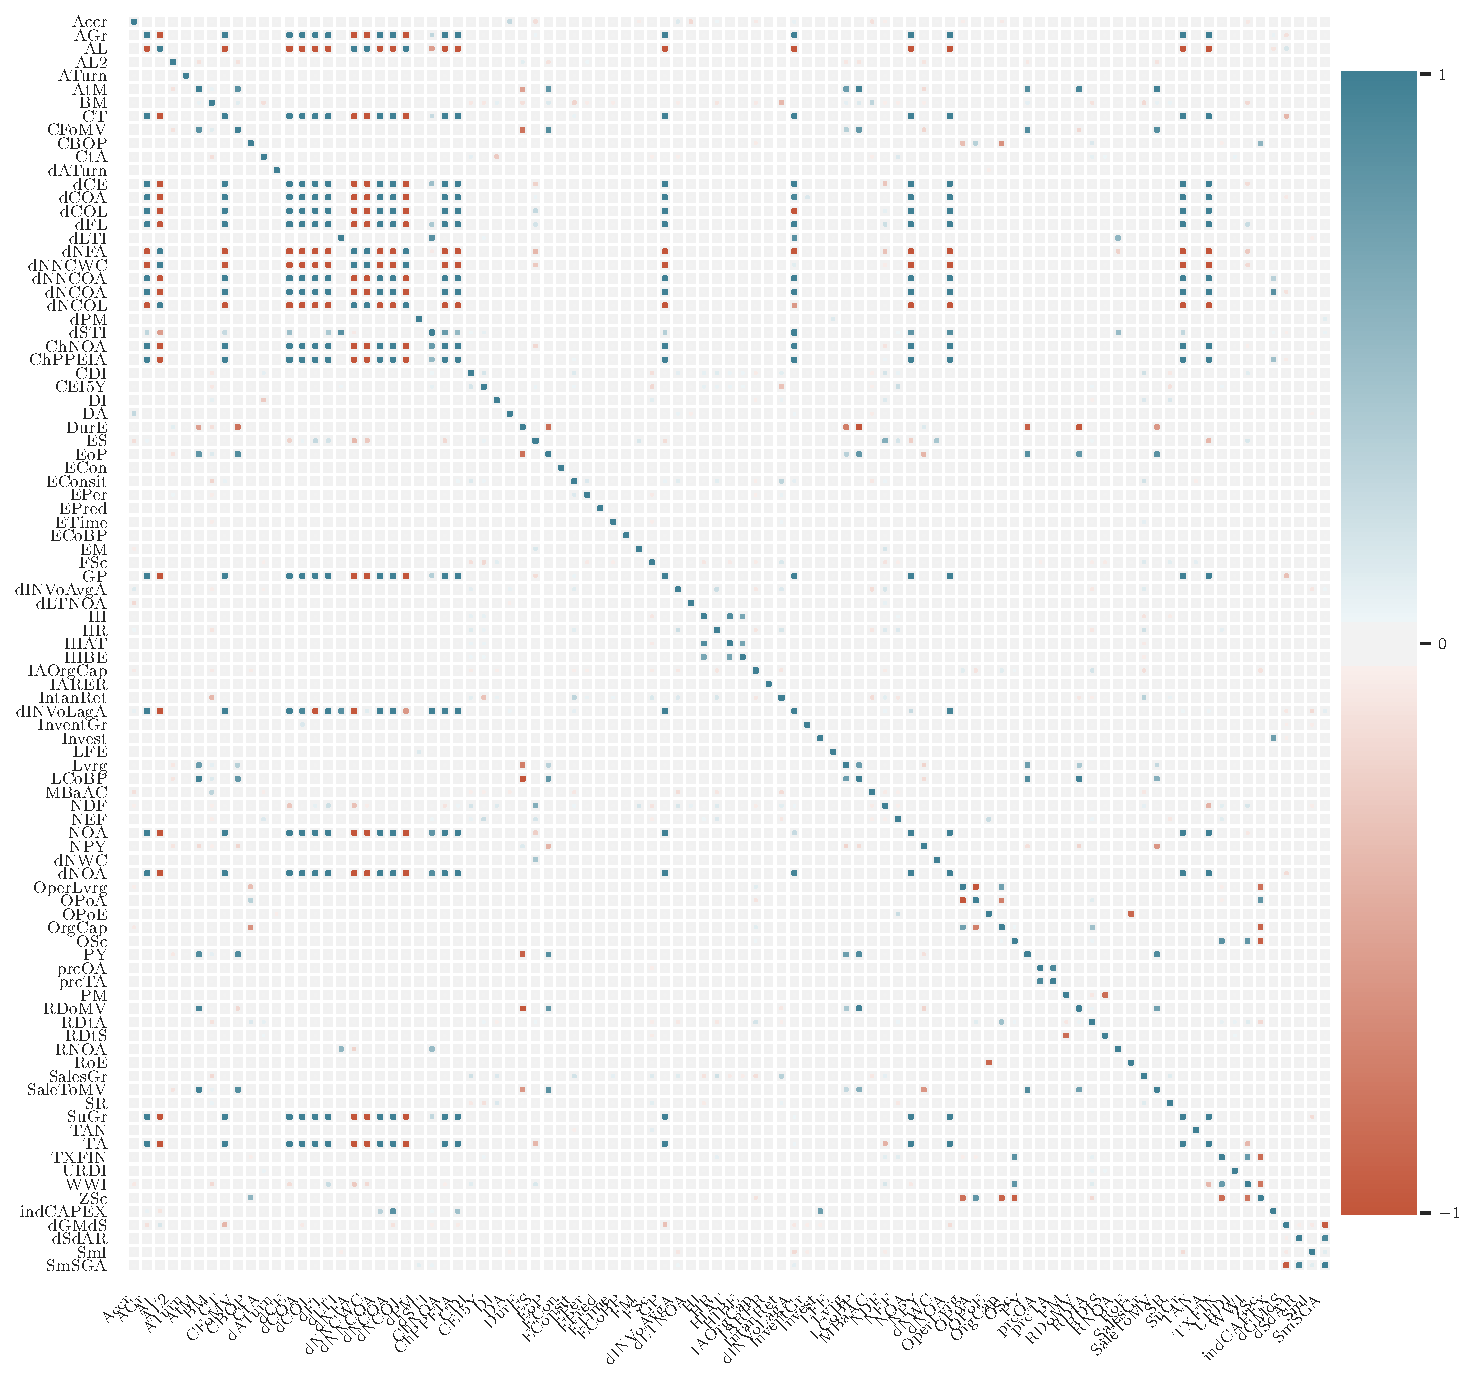
\includegraphics[width=\textwidth,height=\textheight,keepaspectratio]{Figures/corrplot_funds.pdf}
			\caption{Correlation Matrix of Fundamental Anomalies}
			\label{fig:corrplot_funds}
		\end{figure}
	\end{center}
	
	\begin{center}
		\begin{figure}
			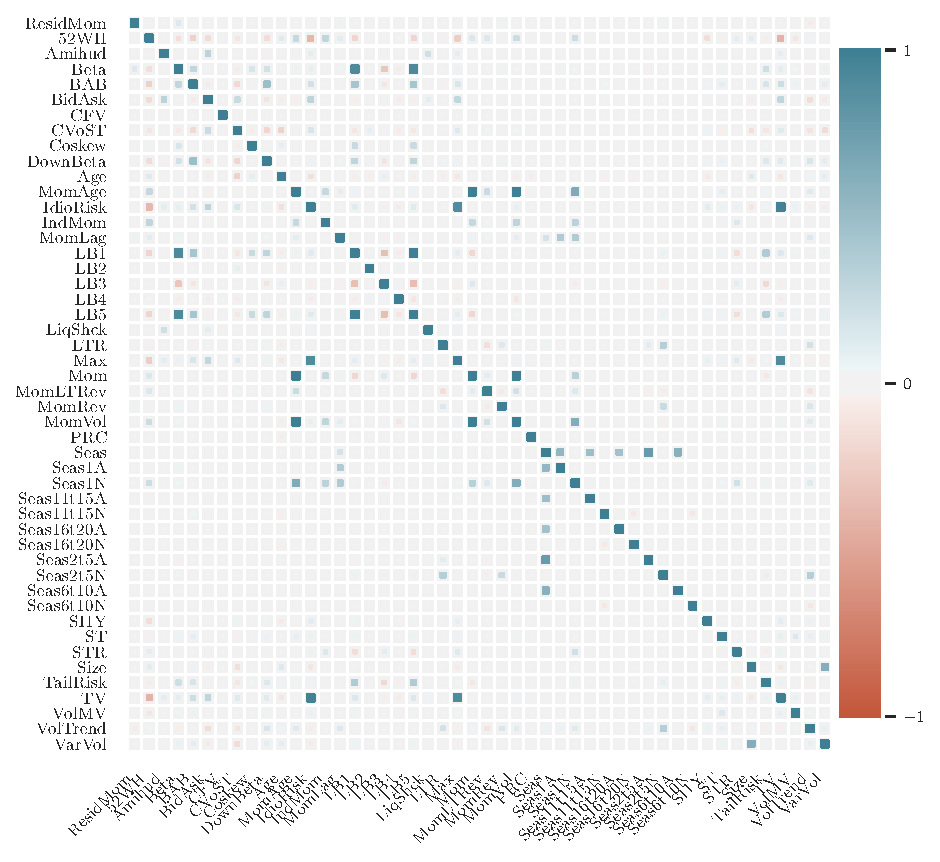
\includegraphics[width=\textwidth,height=\textheight,keepaspectratio]{Figures/corrplot_frictions.pdf}
			\caption{Correlation Matrix of Frictions Anomalies}
			\label{fig:corrplot_frictions}
		\end{figure}
	\end{center}
	
	
	\begin{center}
		\begin{figure}
			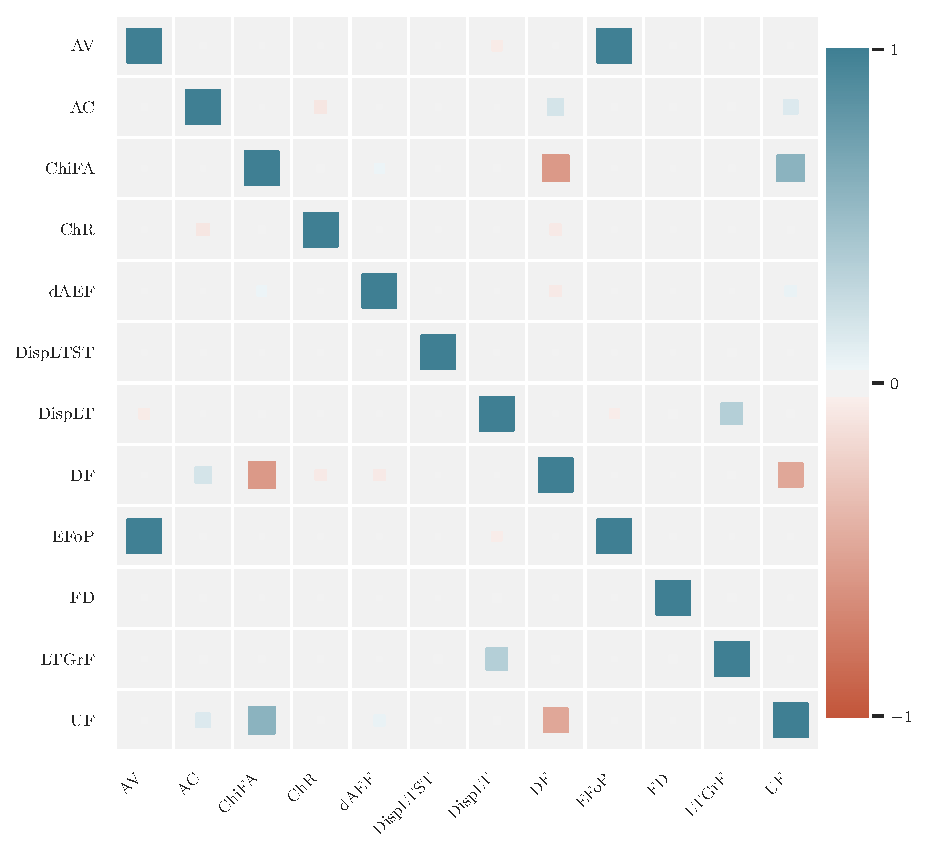
\includegraphics{Figures/corrplot_ibes.pdf}
			\caption{Correlation Matrix of I/B/E/S Anomalies}
			\label{fig:corrplot_ibes}
		\end{figure}
	\end{center}
	
	
	\begin{center}
		\begin{figure}
			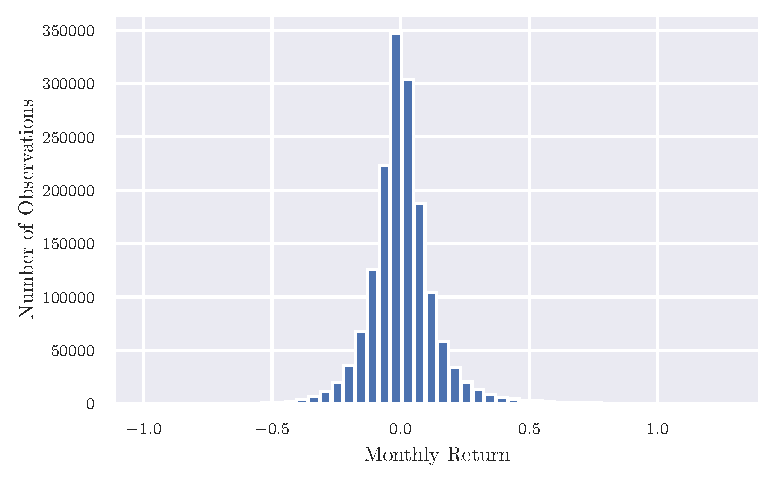
\includegraphics{Figures/hist_returns.pdf}
			\caption{Histogram of Monthly Returns}
			\label{fig:hist_returns}
		\end{figure}
	\end{center}


		
	


